\documentclass{article}
\usepackage{amsmath, amsthm, amssymb, amsfonts}
\usepackage{thmtools}
\usepackage{graphicx}
\usepackage{setspace}
\usepackage{geometry}
\usepackage{float}
\usepackage{hyperref}
\usepackage[utf8]{inputenc}
\usepackage[english]{babel}
\usepackage{framed}
\usepackage[dvipsnames]{xcolor}
\usepackage{tcolorbox}
\usepackage{ dsfont }

\colorlet{LightGray}{White!90!Periwinkle}
\colorlet{LightOrange}{Orange!15}
\colorlet{LightGreen}{Green!15}

\graphicspath{ {./pictures/} }

\newcommand{\HRule}[1]{\rule{\linewidth}{#1}}

% ------------------------------------------------------------------------------

\begin{document}

% ------------------------------------------------------------------------------
% Cover Page and ToC
% ------------------------------------------------------------------------------

\title{ \normalsize \textsc{}
		\\ [2.0cm]
		\HRule{1.5pt} \\
		\LARGE \textbf{\uppercase{ Mathe 2 Hausübung Nr. 5 }
        \HRule{2.0pt} \\ [0.6cm] \LARGE{ Sebastian Steitz, Hannes Albert} \vspace*{10\baselineskip}}
		}
\date{Mai 2023}
\author{\textbf{} \\
		Gruppe:  6\\
		Tutor:  Zidane Bührmann}

\maketitle
\setlength\leftskip{1cm}
\section{H5.1}
\noindent a) \\ 
(i) * Satz 5.10.8 lässt sich umformen in cos(y) = $\sqrt{1 - sin^2(y))}$
\[
    f_1'(y) = arcsin'(y) = \frac{1}{sin'(arcsin(y))} = \frac{1}{cos(arcsin(y))} \overset{*}{=}
    \frac{1}{\sqrt{1-sin^2(arcsin(y))}} = \frac{1}{\sqrt{1-y^2}}
\]
(ii)  
\[
    f_2'(y) = arctan'(y) = \frac{1}{tan'(arctan(y))} = \frac{1}{1 + tan^2(arctan(y))} = \frac{1}{1 + y^2}
\]
(iii) 
\begin{align*}
    f_3(y) = log_2(y) = \frac{ln(y)}{ln(2)} \\ 
    f_3'(y) = \frac{1}{ln(2)} * \frac{1}{y} = \frac{1}{y * ln(2)}
\end{align*}
(iv) 
\[
    f_4'(y) = arctanh'(y) = \frac{1}{1 - tanh^2(arctanh(y))} = \frac{1}{1 - x^2}
\]

\noindent b) \\ 
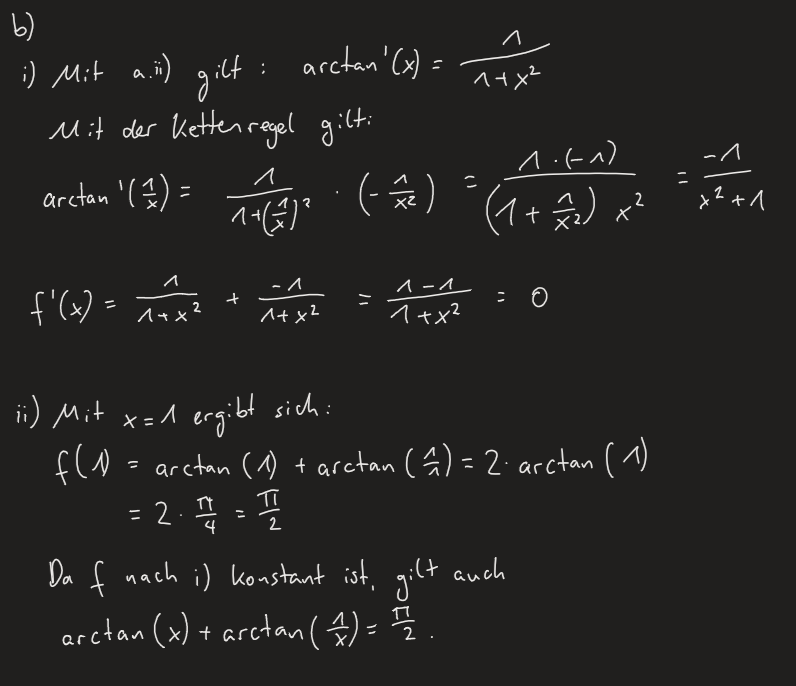
\includegraphics[scale=0.5]{ h1b } \\ 
\bigskip

\section{H5.2}
\noindent a)  

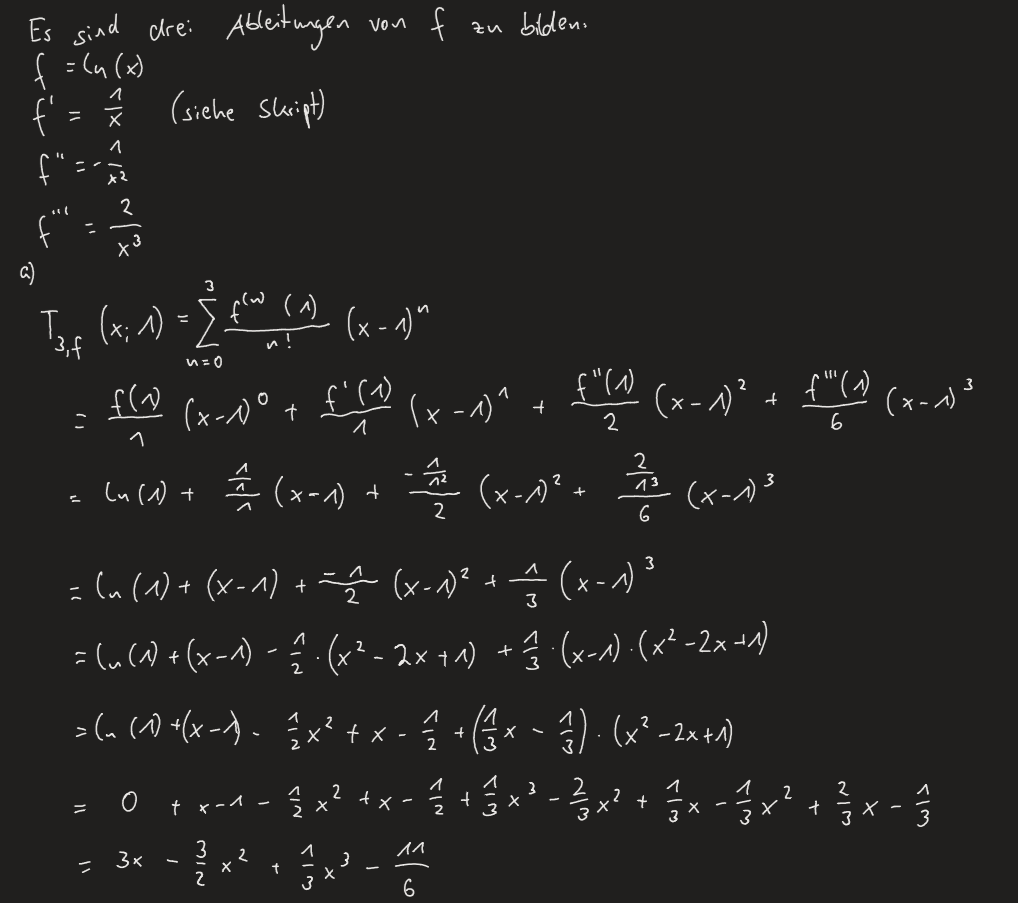
\includegraphics[scale=0.5]{ h2a }  
\newpage
\noindent b) 

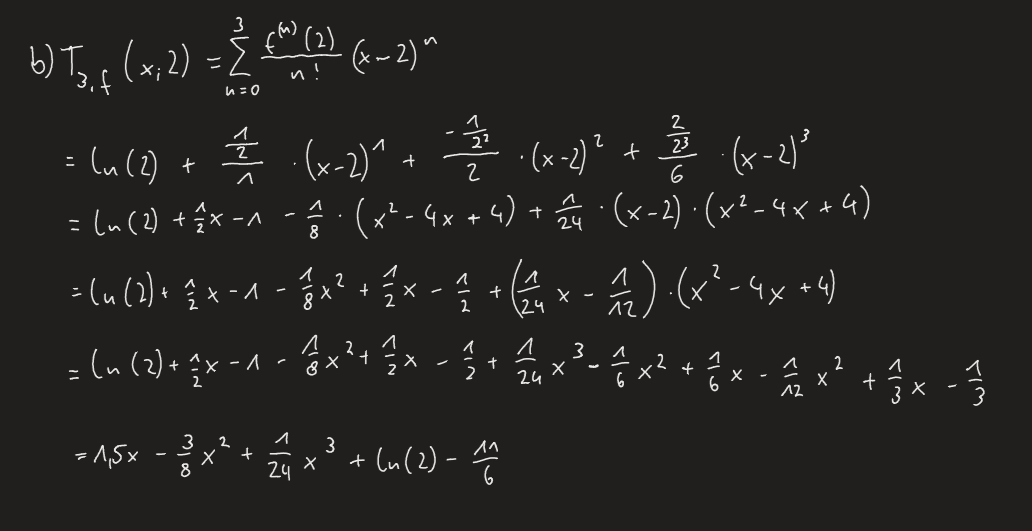
\includegraphics[scale=0.5]{ h2b }  
 
\noindent c)

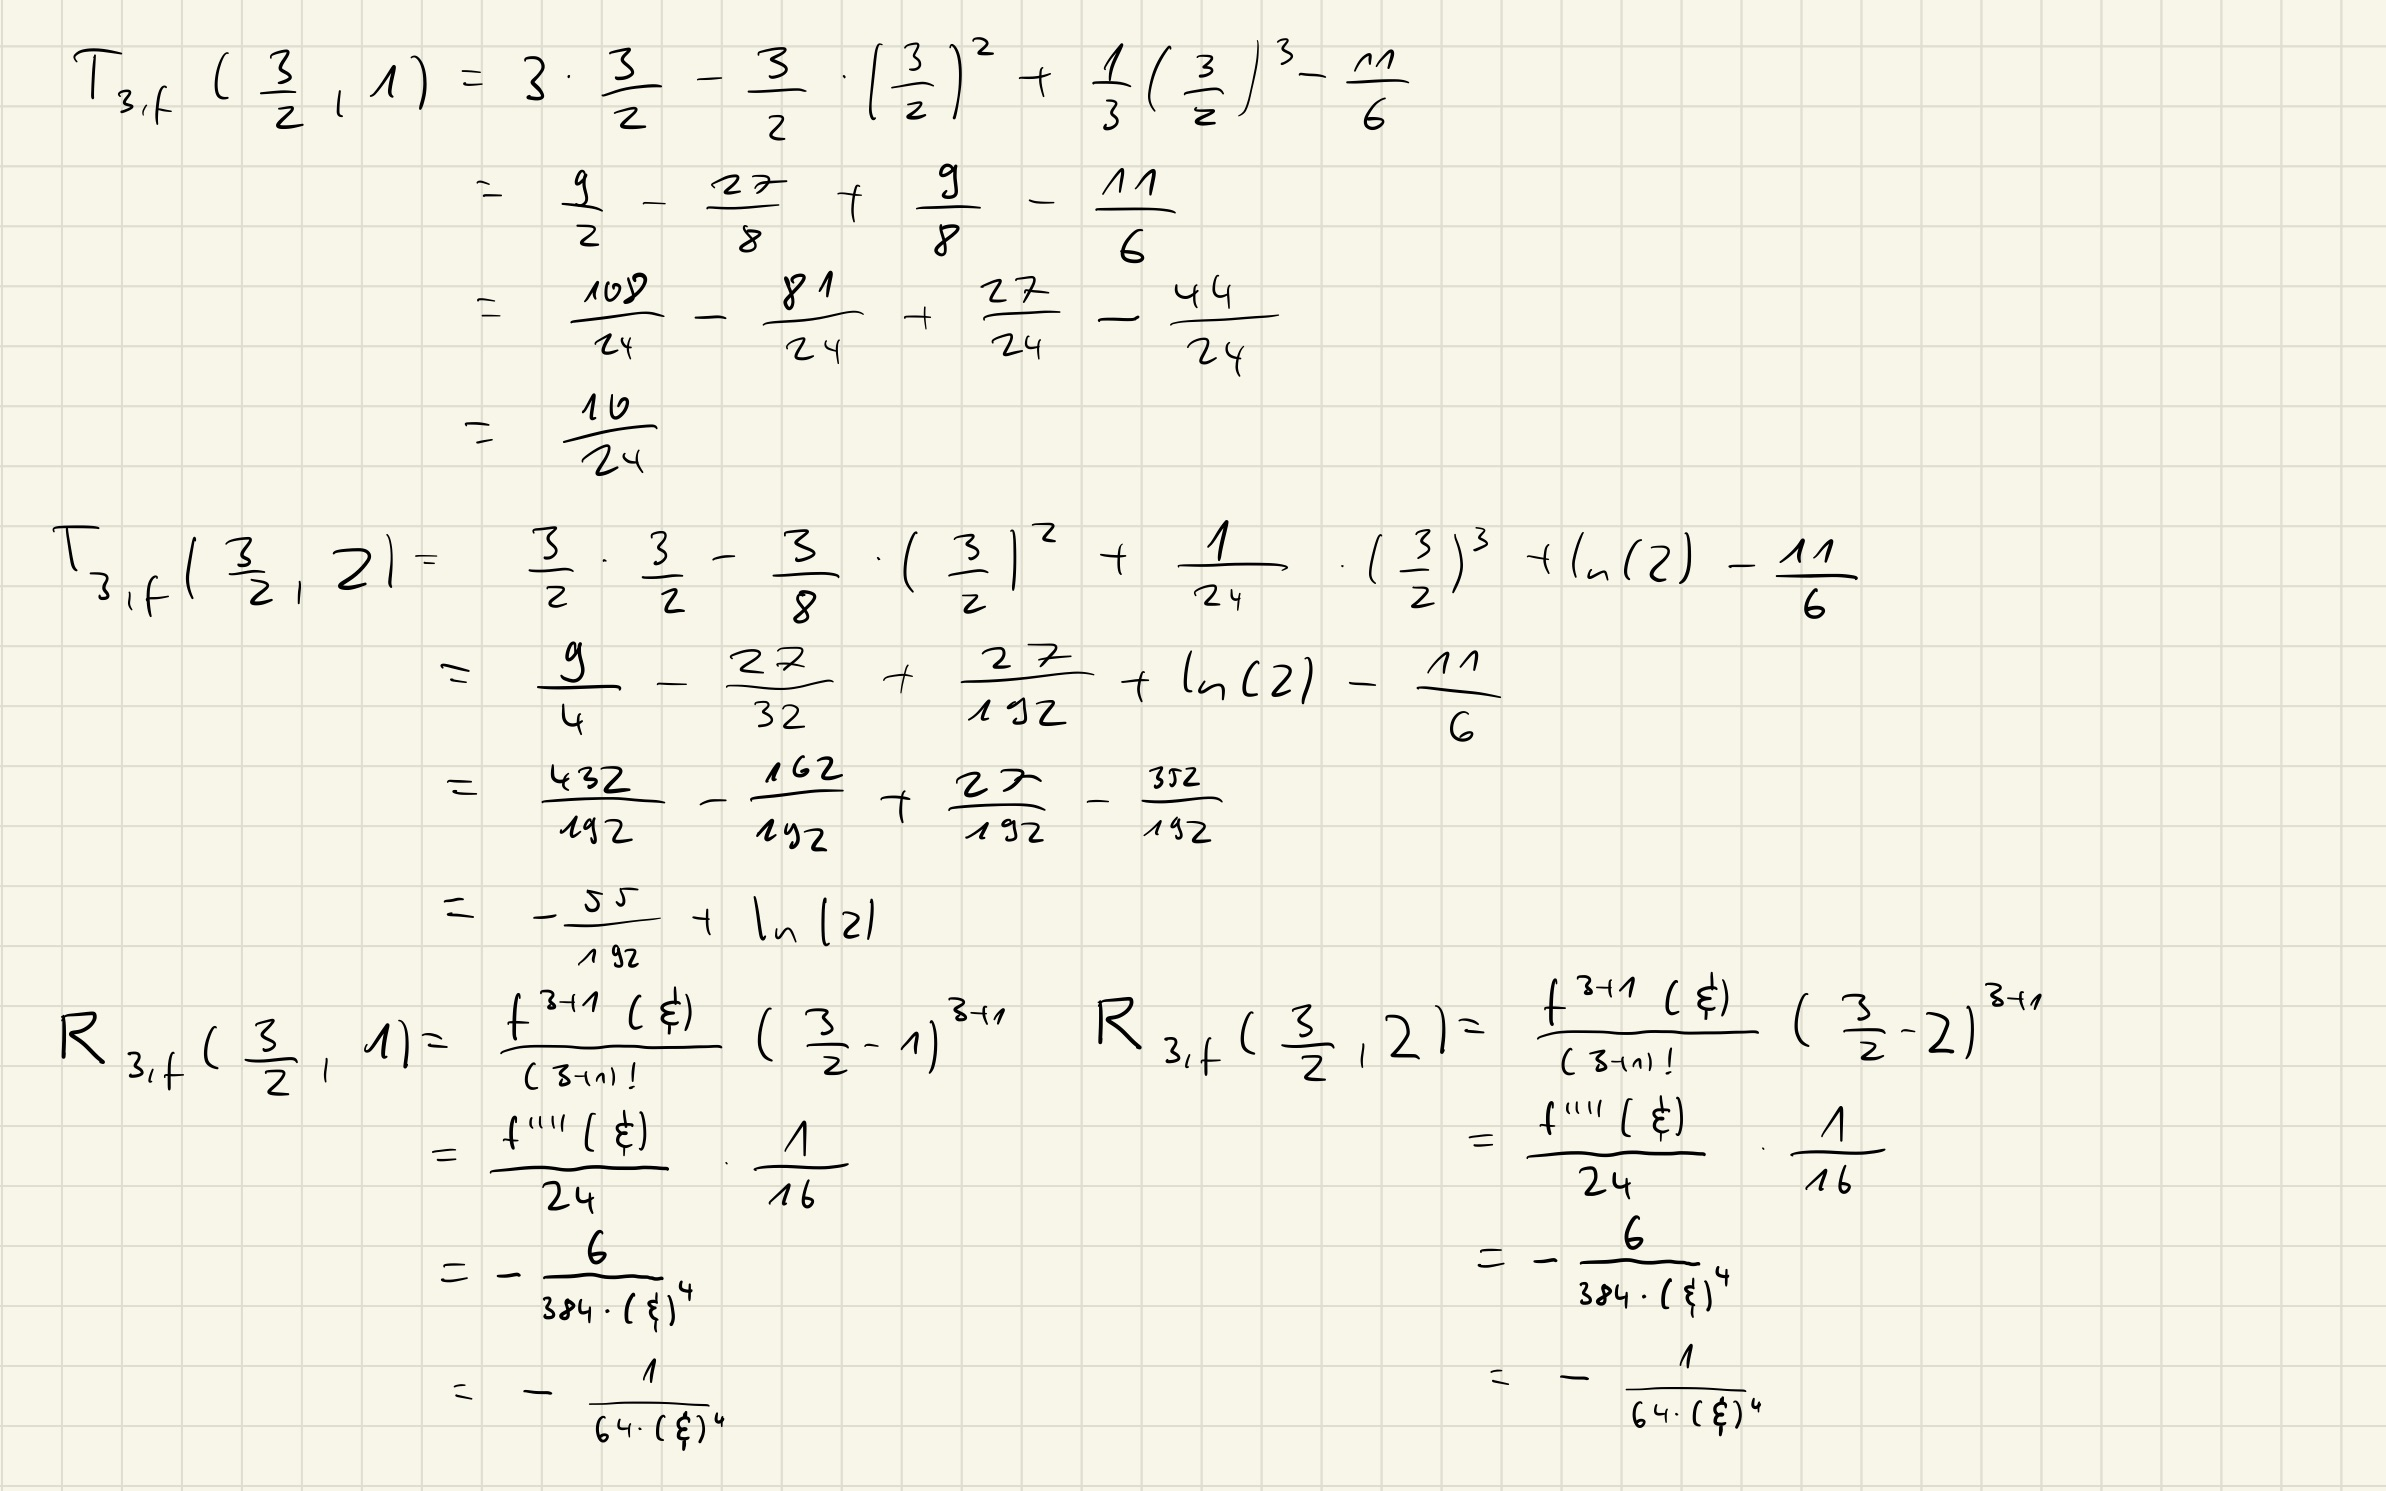
\includegraphics[scale=0.2]{ h2c }  
\newpage
\noindent d) \\ 
Auf drei Nachkommastellen gerundet ist der ln($\frac{3}{2}$) $\approx$ 0.405,
$T_{3, f}(\frac{3}{2}$, 1) $\approx$ 0.417 und  $T_{3, f}(\frac{3}{2}$, 2) 
$\approx$ 0.406. Damit wäre die Approximierung mit $x_0$ = 2 besser.
\end{document}

